\apendice{Plan de Proyecto Software}

\section{Introducción}
El Plan de Proyecto Software describe el proceso de desarrollo de la aplicación web documentada en esta memoria. Describe los procesos seguidos durante la planificación y su seguimiento para el desarrollo continuo del proyecto.
Para la planificación del proyecto se ha usado la aplicación \textbf{Zube}, que permite un seguimiento de las \textit{issues} del repositorio de GitHub que implementa diferentes prácticas ágiles.

Este apartado del Anexo describirá, además, la viabilidad del proyecto, que representa recursos y costes valorados para el mismo, tanto humanos como materiales. Este punto de vista de carácter económico es necesario para conocer los límites del proyecto y saber en qué medida sus objetivos entran dentro de los mismos. Para ello se calculará una aproximación de los fondos que requeriría un trabajador que desarrolle el proyecto, y se valorarán los posibles riesgos surgidos durante el desarrollo y cómo actuar frente a ellos.

Con el enfoque estructurado desarrollado este plan de la documentación, el equipo de desarrollo será capaz de cumplir con los objetivos establecidos del proyecto y entregar un resultado satisfactorio dentro de los límites calculados.

\section{Planificación temporal}
 Como se ha mencionado anteriormente, la planificación temporal del proyecto se ha llevado a cabo con el uso de la herramienta de las \textit{issues} y \textit{milestones} de GitHub, y la herramienta de \textbf{Zube} basando todo el desarrollo en tareas. Cada tarea representa una Issue de GitHub y representan una historia de usuario o pequeña tarea interna. Las tareas están bien estructuradas y clasificadas con etiquetas y \textit{milestones} que indican con qué parte de la estructura del proyecto están relacionadas, y a qué fase del desarrollo pertenecen, respectivamente.

 Un \textit{sprint}, por su parte, representa una fase del desarrollo del software. En la planificación de este proyecto la mayoría de los sprints se han calculado con una duración de dos semanas y han abarcado entre 10 y 18 tareas o \textit{issues}.

 Además, \textbf{Zube} incluye varias herramientas de agilidad que favorecen el seguimiento del desarrollo de la aplicación como los Gráficos \textit{burnup} y \textit{burndown}, que representan la evolución del desarrollo de tareas realizadas en cada \textit{sprint}. Más adelante en esta misma sección se pueden visualizar ejemplos de los gráficos \textit{burndown} resultado de los \textit{sprints}. En la Figura \ref{fig:BurndownS3} se muestra un ejemplo del gráfico \textit{burndown} correspondiente al Sprint 3 - Comparación temporal.
\begin{figure}[H]
\centering
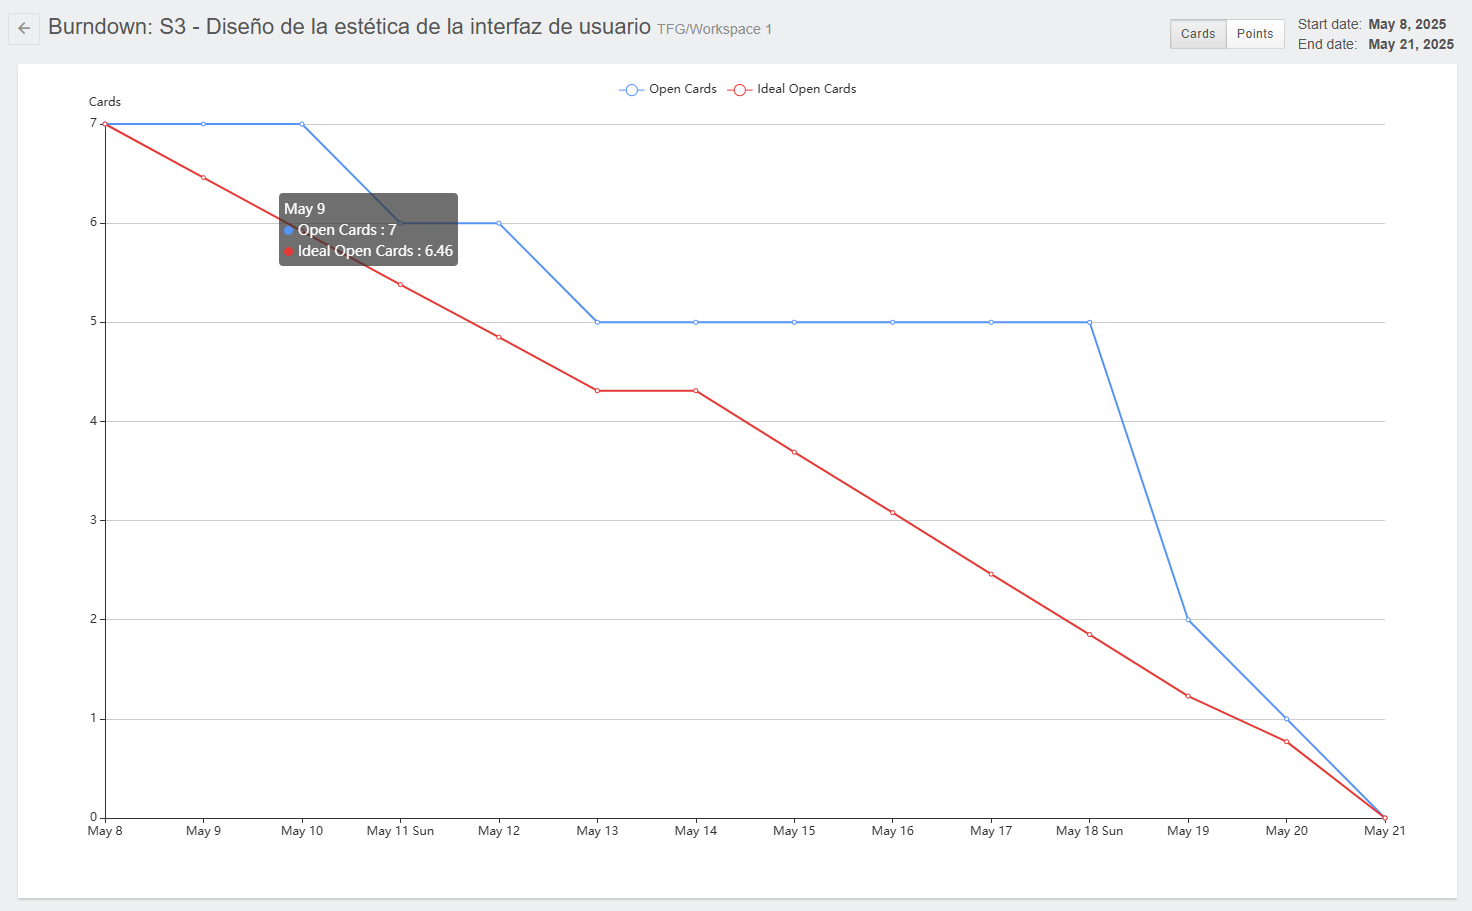
\includegraphics[width=0.8\textwidth]{img/BurndownS3.png}
\caption{Gráfico Burndown del Sprint 3 - Comparación temporal}
\label{fig:BurndownS3}
\end{figure}

 A continuación se explicará cómo se ha desarrollado, por medio de \textit{sprints}, la planificación temporal del proyecto, siguiendo sus respectivas tareas y representando el flujo seguido para la creación y puesta en producción de la aplicación, así como la redacción de esta documentación del proyecto.

 Cada tarea comprendía una historia de usuario o una tarea interna de pequeño tamaño, cuya completación comprende alrededor de un día de duración. 
 En la Figura \ref{fig:Tarea57} se puede observar un ejemplo de tarea en el tablero Kanban de Zube.

\begin{figure}[H]
\centering
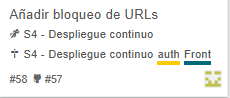
\includegraphics[width=0.8\textwidth]{img/Tarea57.png}
\caption{Ejemplo de una tarea vista en el tablero Kanban de Zube}
\label{fig:Tarea57}
\end{figure}
 
 Los \textit{sprints}, por su parte, han tenido una duración media de quince días, a excepción del primero, pues requirió de varias semanas acordar las bases teóricas y objetivos principales de la aplicación. La Figura \ref{fig:Sprint2} muestra un ejemplo de cómo se visualiza un sprint en Zube.

\begin{figure}[H]
\centering
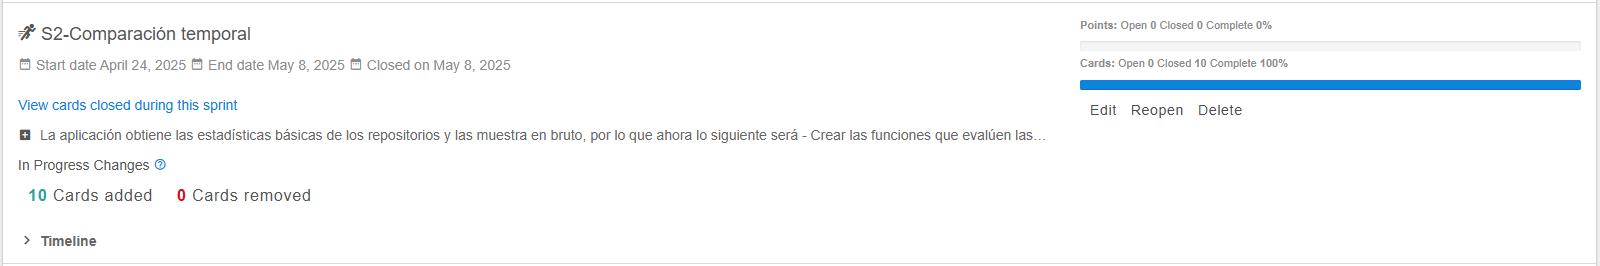
\includegraphics[width=0.8\textwidth]{img/Sprint2.png}
\caption{Ejemplo de un Sprint en Zube}
\label{fig:Sprint2}
\end{figure}

La gestión de las tareas de cada \textit{sprint} ha sido posible gracias a la herramienta del tablero KanBan, que permite gestionar de forma ágil y visual el proceso de desarrollo en el que se encuentra cada tarea. Una tarea se crea y pasa a estado \textit{ready}, preparada para ser comenzada. Una vez esta se empiece a desarrollar, la tarea pasa al estado \textit{in progress}. Una vez terminado el progreso pasará al estado de \textit{in review}, donde se revisará nuevamente el contenido de la tarea para verificar que sea correcto y esté bien implementado, y, en caso positivo, finalizar en el estado \textit{done}, como se puede ver en la siguiente imagen.

\begin{figure}[H]
\centering
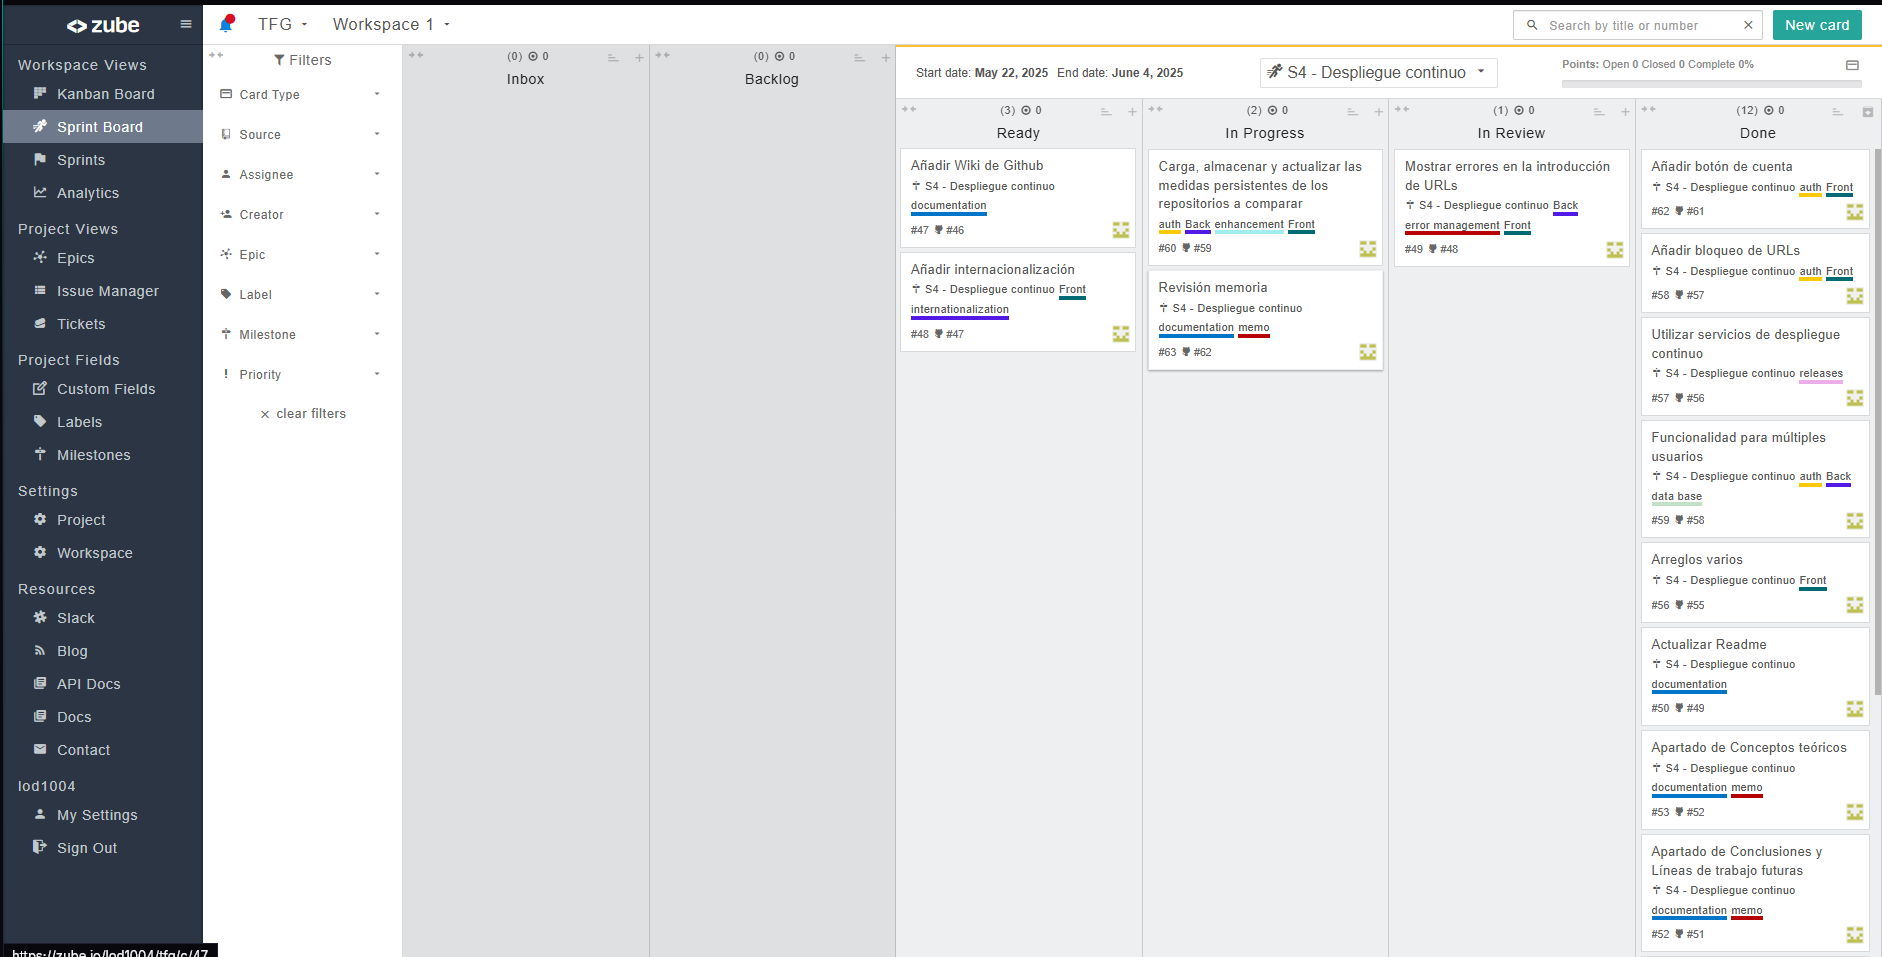
\includegraphics[width=0.8\textwidth]{img/4.1 IteracionZube.png}
\caption{Ejemplo del estado de un sprint visto en el tablero Kanban}
\label{fig:Zube}
\end{figure}

La herramienta de Zube no sólo ha permitido el seguimiento del desarrollo del proyecto en tareas, sino que también ha facilitado la comunicación entre el tutor y el estudiante autor de este TFG, por medio de los comentarios disponibles en cada tarea. Al terminar cada tarea se ha puesto un comentario en la misma indicando los resultados de las actividades asociadas, en ocasiones con imágenes representativas, y el commit que los subió al repositorio del proyecto. Esto ha permitido al tutor exponer su valoración del resultado de la tarea, puntos a mejorar y/o aspectos que necesiten cambios, como se puede ver en la figura \ref{fig:ComentariosTareaZube}

\begin{figure}[H]
\centering
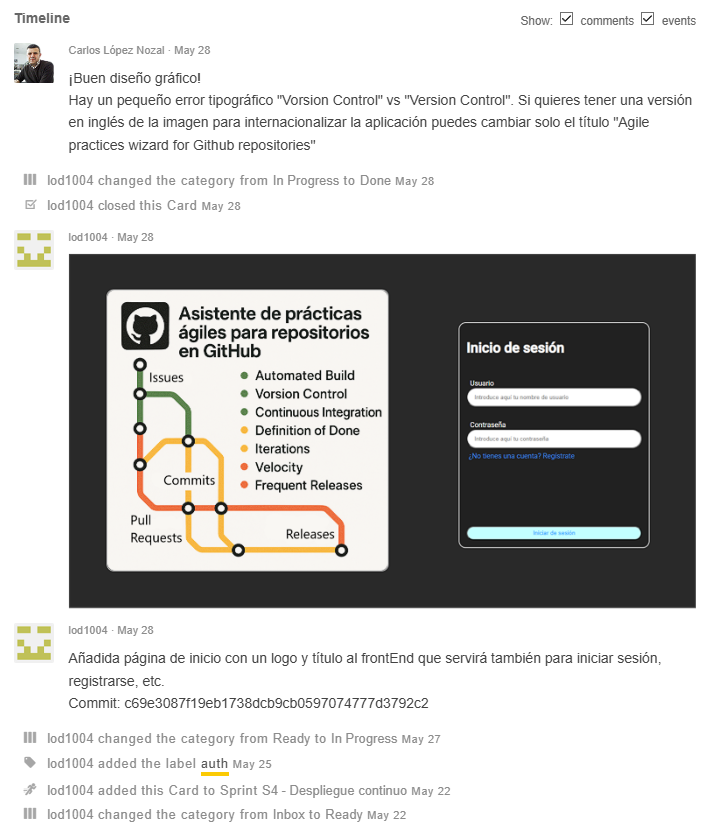
\includegraphics[width=0.8\textwidth]{img/ComentariosTareaZube.png}
\caption{Ejemplo de comentarios en Zube del tutor y alumno en una tarea del proyecto}
\label{fig:ComentariosTareaZube}
\end{figure}

\subsection{Organización en \textit{sprints}}

Para finalizar esta sección se van a desarrollar individualmente los \textit{sprints} definidos y seguidos durante el desarrollo software. Estos \textit{sprints} han sido pensados y creados durante el propio desarrollo en función del estado en el que se encontraba el proyecto, y los objetivos más adecuados que debían ser implementados en cada momento.

\subsubsection{Sprint 0 - Kick-off (1/03/2025 - 03/04/2025)}

Este sprint fue el primero y más largo de todos, pues abarcaría no solo el comienzo del desarrollo del proyecto, sino también la planificación del mismo. Se definió qué aplicación se desarrollaría, sus bases teóricas, el \textit{abstract} y los objetivos principales. Contiene las siguientes 9 tareas:

\begin{enumerate}
\item \textbf{Definir título y descripción del proyecto}: Consistió en, tras terminar de decidir los objetivos y bases del proyecto, redactar el título y descripción iniciales del mismo.
\item \textbf{Introducción del documento}: Redacción inicial del apartado de introducción de la memoria, planteando el contexto y motivación del proyecto.
\item \textbf{Revisión del resumen}: Corrección y mejora del resumen del proyecto, afinando su redacción y adecuación a los objetivos propuestos.
\item \textbf{Anexos}: Preparación de la estructura base de los anexos que acompañarán a la memoria del proyecto.
\item \textbf{Mockups}: Diseño preliminar de la interfaz de usuario para visualizar cómo se estructuraría la aplicación de forma gráfica.
\item \textbf{Definir requisitos funcionales}: Identificación de las funciones clave que debía cumplir la aplicación para alcanzar sus objetivos.
\item \textbf{Rama de pruebas}: Creación de una rama en el repositorio destinada a pruebas y experimentación durante el desarrollo que se usaría en este sprint.
\item \textbf{Estructura del front}: Primer esqueleto del frontend de la aplicación, estableciendo la organización interna de los componentes básicos.
\item \textbf{Estructura del back}: Configuración inicial del backend y definición de su arquitectura básica.
\end{enumerate}

\begin{figure}[H]
\centering
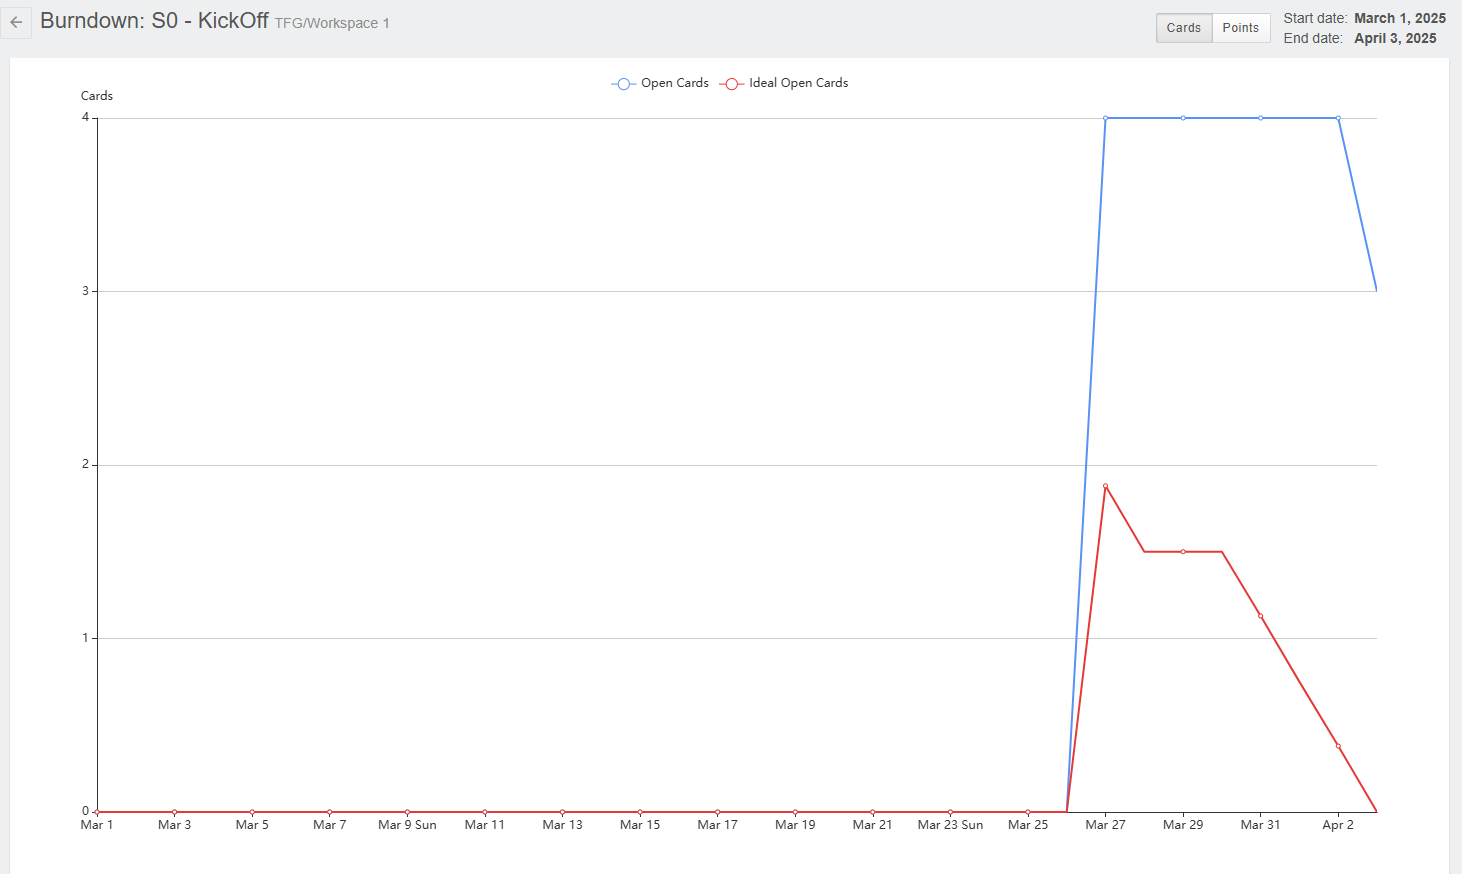
\includegraphics[width=0.8\textwidth]{img/BurndownS0.png}
\caption{Gráfico Burndown del Sprint 0 - Kick-off}
\label{fig:BurndownS0}
\end{figure}

\subsubsection{Sprint 1 - Primer prototipo de la aplicación (8/04/2025 - 22/04/2025)}

Instaladas las herramientas básicas del proyecto y asentadas las ideas del mismo, comienza el desarrollo con un pequeño prototipo de la aplicación. Se perseguían los siguientes objetivos: conectar el backend con el frontend, definir las reglas que se evaluarán, continuar con la documentación y realizar los primeros análisis de datos.

\begin{enumerate}
\item \textbf{Conexión Front - Back}: Establecimiento de la comunicación entre el frontend y el backend.
\item \textbf{Recogida de Repositorio vía URL}: Implementación de una funcionalidad para introducir un repositorio mediante su URL.
\item \textbf{Guardar repositorio en base de datos}: Añadir la funcionalidad de almacenamiento de repositorios para su análisis posterior.
\item \textbf{Recoger número de Issues abiertas y cerradas}: Desarrollo de una métrica base para evaluar las \textit{issues} del repositorio.
\item \textbf{Mostrar número de Issues}: Visualización en la interfaz del número de \textit{issues}, como parte de las estadísticas presentadas.
\item \textbf{Evaluar mensajes de los commits}: Análisis del contenido de los mensajes de los commits para detectar buenas prácticas.
\item \textbf{Evaluar Issues en el tiempo}: Cálculo de métricas temporales sobre la evolución de los \textit{issues}.
\item \textbf{Evaluar Pull Requests}: Análisis de la actividad de las \textit{pull requests} como indicador de colaboración.
\item \textbf{Evaluar Releases}: Inclusión de información sobre las versiones liberadas del proyecto.
\item \textbf{Evaluar Acciones}: Estudio de las GitHub Actions empleadas como parte del flujo de trabajo.
\item \textbf{Definir reglas}: Redacción y codificación de las reglas de evaluación de buenas prácticas basadas en metodología ágil.
\end{enumerate}

\begin{figure}[H]
\centering
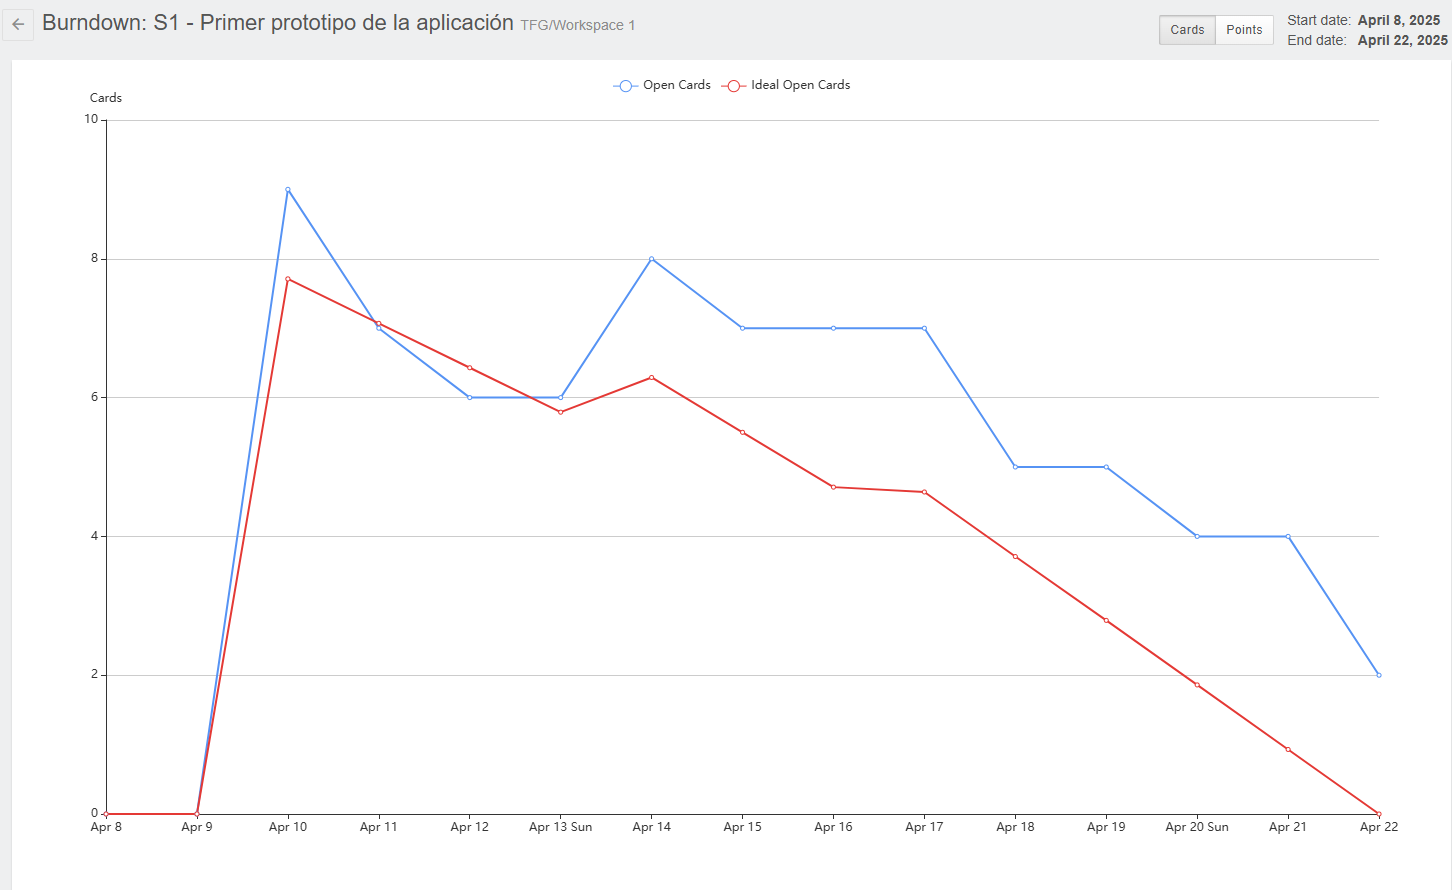
\includegraphics[width=0.8\textwidth]{img/BurndownS1.png}
\caption{Gráfico Burndown del Sprint 1 - Primer prototipo de la aplicación}
\label{fig:BurndownS1}
\end{figure}

\subsubsection{Sprint 2 - Comparación temporal (24/04/2025 - 08/05/2025)}

La aplicación ya obtiene estadísticas básicas. En este sprint se centró en implementar una comparación temporal entre repositorios, añadir control de errores y documentar la evolución temporal de los proyectos.

\begin{enumerate}
\item \textbf{Crear funciones de las reglas}: Implementación concreta de las funciones para evaluar las reglas definidas.
\item \textbf{Mostrar cumplimiento de reglas}: Inclusión en el frontend de indicadores que muestran si se cumplen las reglas.
\item \textbf{Extraer intervalos de tiempo del repositorio}: Implementar la funcionalidad de los intervalos de tiempo para comparar la actividad del repositorio.
\item \textbf{Selección de intervalos de tiempo}: Interfaz para que el usuario pueda seleccionar intervalos de tiempo a usar en el análisis.
\item \textbf{Añadir estadísticas temporales}: Implementación de métricas que reflejen la evolución cada cierto número de días.
\item \textbf{Añadir estadísticas restantes}: Inclusión de estadísticas que aún no habían sido implementadas.
\item \textbf{Estadísticas de participantes}: Incorporación de datos sobre los miembros del repositorio.
\item \textbf{Ordenar Base de datos}: Refactorización y optimización de la estructura de almacenamiento de repositorios y medidas de calidad de proceso.
\item \textbf{Añadir control de errores}: Añadir gestión de errores para situaciones como problemas de red o repositorios no válidos.
\item \textbf{Documentar sobre la evolución de proyectos en el tiempo}: Redacción teórica en la memoria sobre las fases de un proyecto ágil.
\end{enumerate}

\begin{figure}[H]
\centering
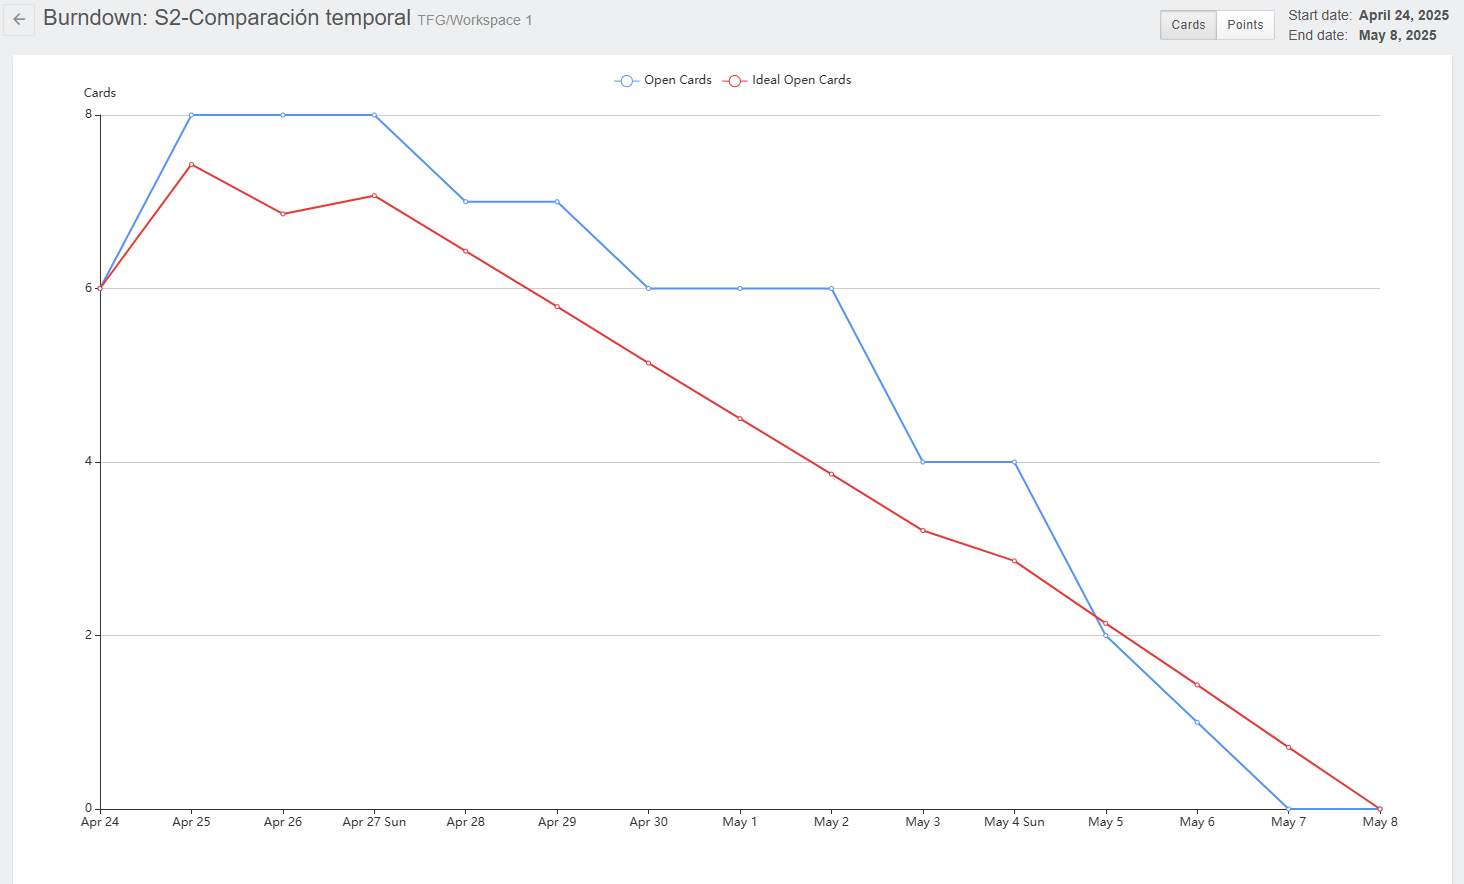
\includegraphics[width=0.8\textwidth]{img/BurndownS2.png}
\caption{Gráfico Burndown del Sprint 2 - Comparación temporal}
\label{fig:BurndownS2}
\end{figure}

\subsubsection{Sprint 3 - Diseño de la estética de la interfaz de usuario (08/05/2025 - 21/05/2025)}

Con una versión funcional disponible, se procedió a mejorar la experiencia de usuario y seguir avanzando en la documentación del proyecto. El principal objetivo era maquetar la interfaz de usuario para que esta se pareciera al \textit{mockup} diseñado en el Sprint 0 - KickOff.

\begin{figure}[H]
\centering
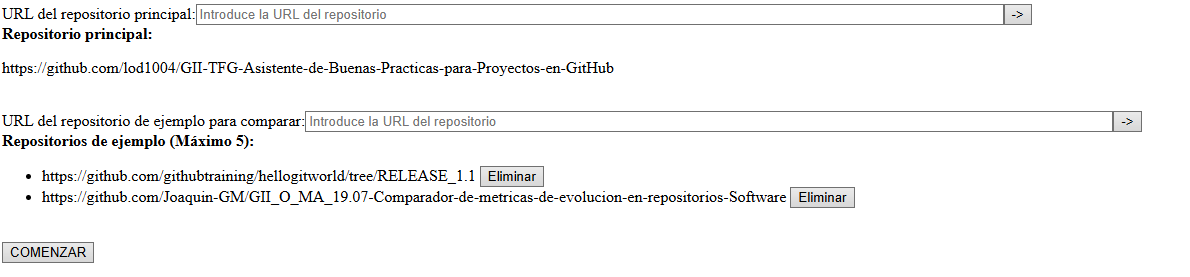
\includegraphics[width=0.8\textwidth]{img/Interfaz inicial.png}
\caption{Imagen de la primera versión de la interfaz de la aplicación}
\label{fig:Interfaz inicial}
\end{figure}

\begin{figure}[H]
\centering
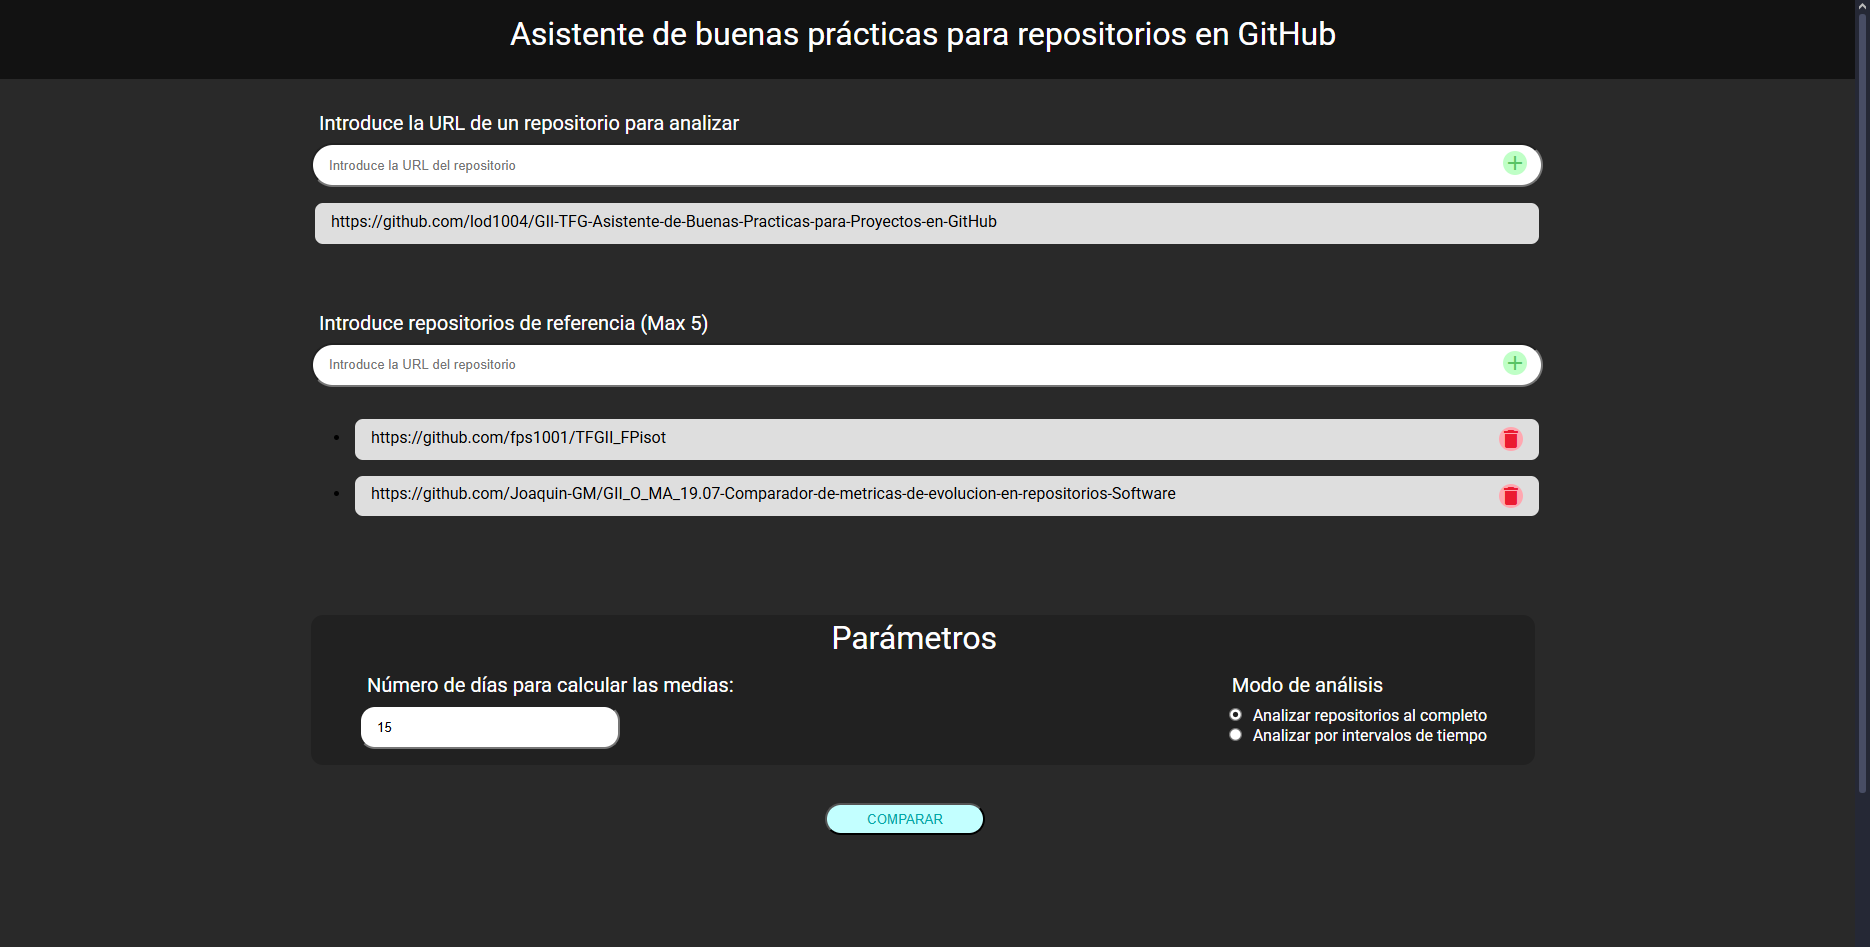
\includegraphics[width=0.8\textwidth]{img/Interfaz intermedia.png}
\caption{Imagen de la interfaz tras la maquetación del Sprint 3 - Diseño de la estética de la interfaz de usuario}
\label{fig:Interfaz intermedia}
\end{figure}

Como se puede apreciar en las figuras \ref{fig:Interfaz inicial} y \ref{fig:Interfaz intermedia}, este Sprint supuso un cambio significado para el diseño de la interfaz de usuario, y el \textit{look and feel} de la aplicación.

\begin{enumerate}
\item \textbf{Maquetación del FrontEnd}: Rediseño visual del frontend para mejorar la experiencia y estética.
\item \textbf{Nuevas estadísticas y revisión}: Mejora de algunas métricas, añadido de alguans nuevasy validación de los resultados obtenidos.
\item \textbf{Añadir Spinner}: Mejora visual mediante un componente que indica la carga de información.
\item \textbf{Implementar logs}: Sistema de registro de eventos para facilitar el mantenimiento.
\item \textbf{Información sobre resultados de las reglas}: Mostrar explicaciones detalladas de cada regla y su resultado.
\item \textbf{Apartado de "Trabajos Relacionados"}: Redacción del apartado que contextualiza el trabajo con investigaciones previas.
\item \textbf{Apartado de "Aspectos relevantes del desarrollo"}: Inclusión en la memoria de las decisiones clave durante el desarrollo.
\item \textbf{Apartado de "Objetivos del proyecto"}: Definición clara de los objetivos concretos que se querían alcanzar.
\item \textbf{Apartado de "Técnicas y herramientas"}: Descripción de las herramientas usadas y su justificación.
\item \textbf{Primera Release del proyecto}: Publicación de la primera versión oficial v0.1.0 de la aplicación.
\end{enumerate}

\begin{figure}[H]
\centering
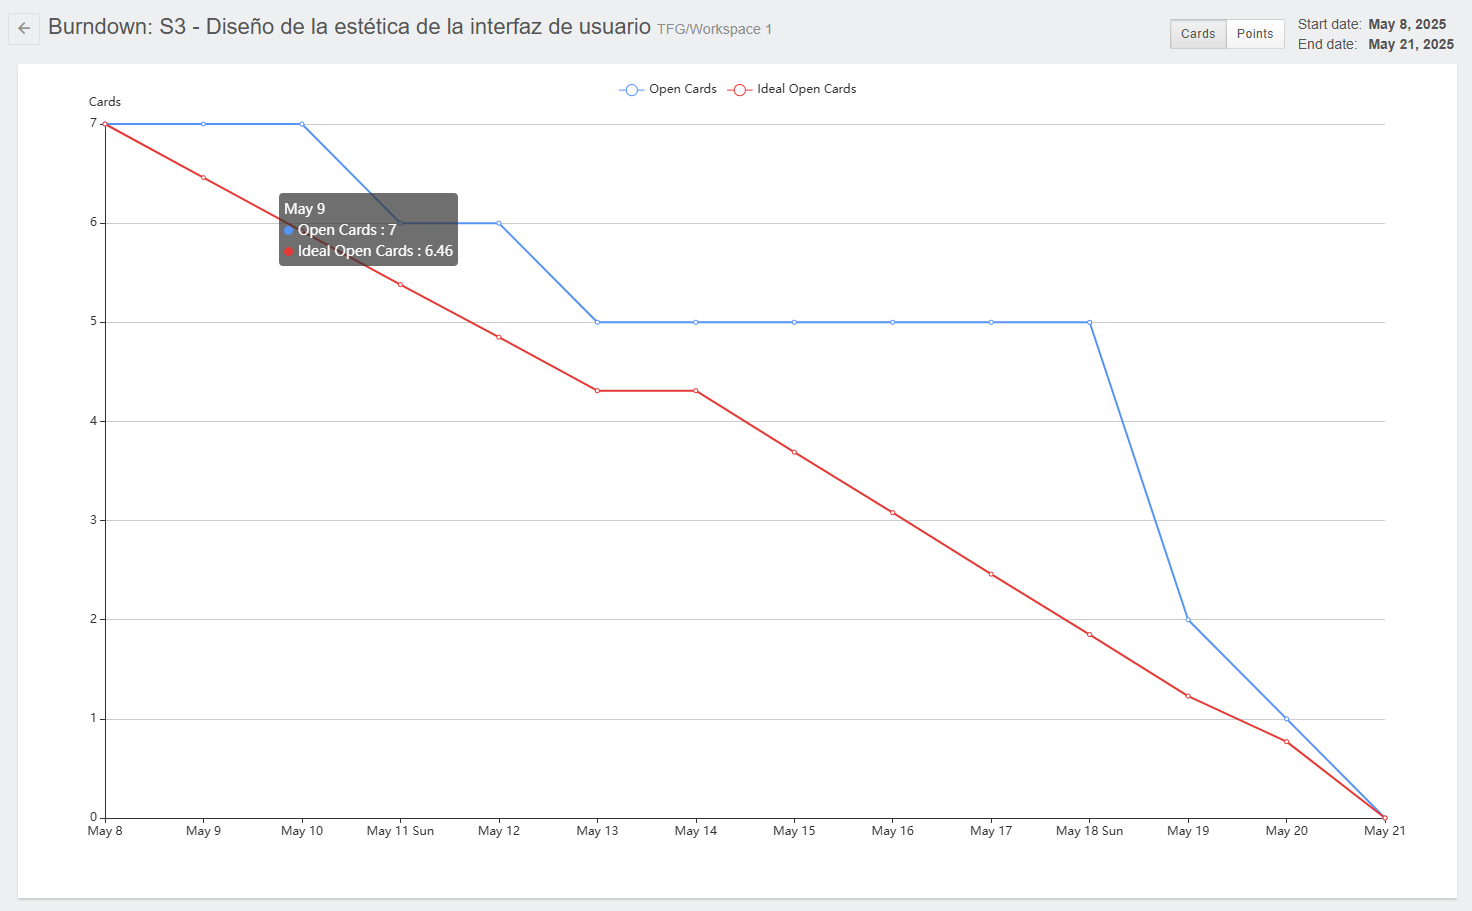
\includegraphics[width=0.8\textwidth]{img/BurndownS3.png}
\caption{Gráfico Burndown del Sprint 3 - Diseño de la estética de la interfaz de usuario}
\label{fig:BurndownS3}
\end{figure}

\subsubsection{Sprint 4 - Despliegue continuo (22/05/2025 - 09/06/2025)}

En este último sprint se trabajó en el despliegue de la aplicación, correcciones finales, soporte para múltiples usuarios y finalización de la memoria.

\begin{enumerate}
\item \textbf{Utilizar servicios de despliegue continuo}: Implementación de un flujo de despliegue automático tras cada actualización.
\item \textbf{Mostrar errores en la introducción de URLs}: Validación del input del usuario para evitar URLs no válidas.
\item \textbf{Añadir internacionalización}: Soporte para diferentes idiomas en la interfaz de usuario.
\item \textbf{Añadir página de inicio}: Creación de una landing page para la aplicación que serviría como formulario de login.
\item \textbf{Cambiar título y nomenclaturas}: Revisión de nombres de variables y componentes para mayor claridad.
\item \textbf{Actualizar Readme}: Actualización de la documentación principal del repositorio con instrucciones claras.
\item \textbf{Añadir Wiki de Github}: Creación de una wiki complementaria al README para documentar el uso.
\item \textbf{Añadir usuarios y login}: Implementación básica de autenticación de usuarios.
\item \textbf{Funcionalidad para múltiples usuarios}: Adaptación del backend para permitir análisis separados por usuario.
\item \textbf{Añadir botón de cuenta}: Crear un botón de apertura del menú de usuario.
\item \textbf{Revisión memoria}: Revisión general del contenido escrito de la memoria.
\item \textbf{PDF completo de la memoria}: Generación del documento final completo en formato PDF.
\item \textbf{Apartado de Conclusiones y Líneas de trabajo futuras}: Reflexión final sobre el proyecto y posibles continuaciones en la memoria.
\item \textbf{Apartado A de los anexos}: Redacción del apartado A de los anexos.
\item \textbf{Revisión del apartado B de los anexos}: Revisión del apartado B de los anexos.
\item \textbf{Apartado C de los anexos}: Redacción del apartado C de los anexos.
\item \textbf{Apartado D de los anexos}: Redacción del apartado D de los anexos.
\item \textbf{Apartado E de los anexos}: Redacción del apartado E de los anexos.
\item \textbf{Apartado F de los anexos}: Redacción del apartado F de los anexos.
\item \textbf{Anexos (finales)}: Inclusión de todos los anexos restantes con los elementos complementarios.
\item \textbf{Test eficiencia v.0.2.0}: Evaluación de la eficiencia del sistema tras la última versión.
\item \textbf{Arreglos varios}: Correcciones menores y ajustes visuales o funcionales.
\end{enumerate}

\begin{figure}[H]
\centering
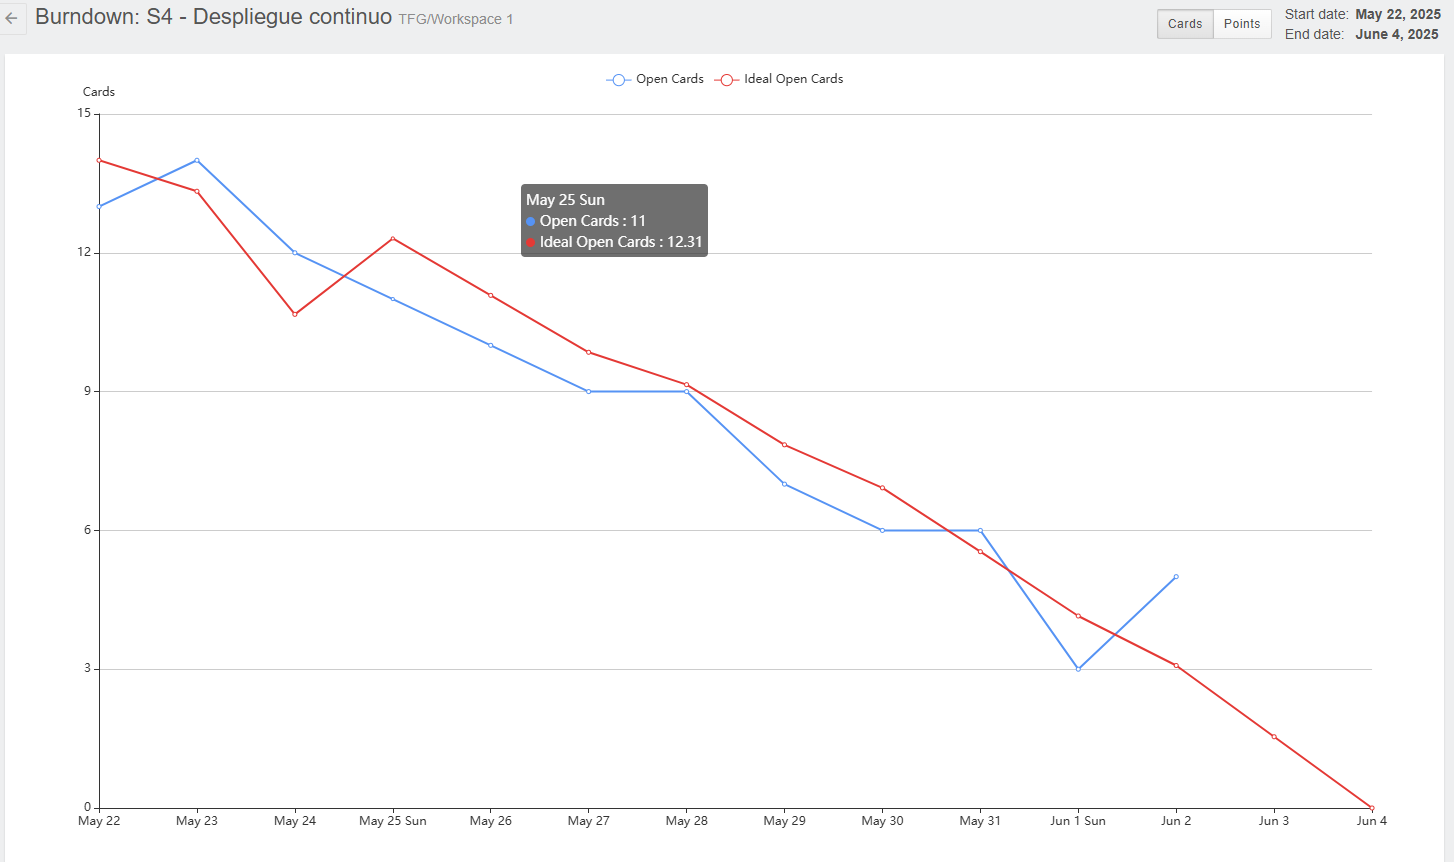
\includegraphics[width=0.8\textwidth]{img/BurndownS4.png}
\caption{Gráfico Burndown del Sprint 4 - Despliegue continuo}
\label{fig:BurndownS4}
\end{figure}

\section{Estudio de viabilidad}

Este apartado recoge un análisis detallado sobre la viabilidad del proyecto desde una doble perspectiva: económica y legal. Se examinan los recursos necesarios para el desarrollo de la aplicación web \textbf{Asistente de prácticas ágiles para repositorios en GitHub} en equipos de desarrollo que utilizan GitHub, así como los requisitos y restricciones legales que podrían condicionar su puesta en marcha. Dado su enfoque académico, automatizado y extensible, el proyecto se plantea como una herramienta útil tanto para entornos académicos como profesionales, y su desarrollo es asumido por un único responsable técnico.

\subsection{Viabilidad económica}

\subsubsection{Costes de personal}

El desarrollo ha sido asumido por una sola persona con perfil de estudiante de ingeniería informática. De acuerdo con el XVIII Convenio Colectivo Estatal de Empresas de Consultoría y Tecnologías de la Información \cite{boe2023_consultoria}, se estima un coste bruto mensual en torno a 2.000 €. Para el desarrollo completo del proyecto se contemplan hasta 4 meses de trabajo.

\tablaSmallSinColores
{Costes de \textit{personal}}
{lc}
{costes-personal}
{%
	\textbf{Concepto} & \textbf{Coste} \\
}
{%
	Salario mensual & 1.500€ \\
	Seguridad Social y retenciones & 500€ \\
	\midrule
	\textbf{Total 4 meses} & \textbf{8.000€} \\
}

\subsubsection{Coste de hardware}

Se presupone la utilización de un equipo de sobremesa ya disponible con prestaciones suficientes para ejecutar herramientas de desarrollo, e instalar aplicaciones y herramientas de programación y puesta en producción, así como entornos de inferencia local. A efectos contables, se considera una amortización del equipo a 3 años.

\tablaSmallSinColores
{Costes de \textit{hardware}}
{lcc}
{costes-hardware}
{%
	\textbf{Concepto} & \textbf{Coste} & \textbf{Coste amortizado} \\
}
{%
	Ordenador de desarrollo & 500€ & 113€ \\
	\midrule
	\textbf{Total} & \textbf{500€} & \textbf{113€} \\
}

\subsubsection{Coste de conectividad}

El uso continuo de internet es fundamental, tanto para descargar dependencias como para utilizar APIs de inferencia o conectarse a servicios de terceros como GitHub\cite{github_docs}, Vercel\cite{vercel_platform} o Render\cite{render_platform}. Se estima un coste medio mensual de 35€.

\begin{itemize}
	\item \textbf{Total en conectividad (4 meses):} 140€
\end{itemize}

\subsubsection{Coste de software}

Todo el software utilizado en el desarrollo es de código abierto o con licencias gratuitas para su uso individual: Visual Studio Code, GitHub, Vercel (usando entornos públicos gratuitos) y Render. El sistema operativo empleado es Windows 10 Home, de un coste de alrededor de 10 euros y ampliamente compatible con las herramientas mencionadas.

\textbf{Coste estimado: 10€}

\subsubsection{Auditoría y supervisión académica}

Se reserva un coste temporal asociado al seguimiento del proyecto por parte del tutor, que incluye la corrección del código, revisión de entregables y reuniones de orientación técnica.

\tablaSmallSinColores
{Costes totales del asistente inteligente para prácticas ágiles}
{lc}
{costes-totales}
{%
	\textbf{Concepto} & \textbf{Coste} \\
}
{%
	Mano de obra & 8.000€ \\
	Hardware amortizado & 113€ \\
	Conectividad & 140€ \\
	Software Windows 10 & 10€ \\
	Revisión académica & 750€ \\
	\midrule
	\textbf{Total} & \textbf{9.306€} \\
}

\subsubsection{Sostenibilidad económica del proyecto}

Una vez completado el desarrollo inicial, el coste de mantenimiento es bajo, especialmente si se utilizan modelos locales. La monetización del asistente podría basarse en:

\begin{itemize}
	\item \textbf{Licencia freemium:} acceso básico gratuito y funciones avanzadas bajo suscripción.
	\item \textbf{Integración en GitHub Marketplace:} cobro por instalación en organizaciones.
	\item \textbf{Modelo educativo:} cesión gratuita a universidades con apoyo institucional.
\end{itemize}

\subsection{Viabilidad legal}

\subsubsection{Licencias del software utilizado}

Se ha garantizado el uso exclusivo de herramientas de código abierto o con licencias permisivas  Esto incluye tanto las librerías públicas usadas en el frontend y el backend como herramientas de despliegue continuo como Vercel o Render

\begin{itemize}
	\item Librerías de Angular y Node.js.
	\item Integraciones continuas con GitHub, Vercel y Render.
\end{itemize}

\subsubsection{Términos de uso de las APIs de terceros}

Al utilizar servicios de inferencia por API (En este caso GitHub API) deben respetarse las políticas de uso responsable, límites de almacenamiento de datos y uso no comercial sin licencia explícita.

\textbf{Requisitos:}

\begin{itemize}
	\item Consentimiento del usuario en el tratamiento de repositorios.
	\item Prohibición del reentrenamiento sobre inputs sin autorización.
\end{itemize}

\subsubsection{Protección de datos}

En caso de desplegar el asistente en organizaciones reales, será necesario cumplir con la normativa de protección de datos como el RGPD:

\begin{itemize}
	\item Anonimización de inputs del usuario.
	\item Consentimiento explícito para recoger métricas.
	\item Política de privacidad visible.
\end{itemize}

\subsubsection{Restricciones de publicación}

Si el asistente se publica en plataformas como GitHub Marketplace o se distribuye como SaaS, deberá incluir:

\begin{itemize}
	\item Condiciones de uso claras.
	\item Política de privacidad.
	\item Declaración de uso de APIs externas.
\end{itemize}

\subsubsection{Checklist legal}

\begin{enumerate}
	\item Verificación de licencias de todas las librerías.
	\item Inclusión de política de privacidad si se recoge algún dato.
	\item Revisión de los términos de cada API externa usada.
	\item Consentimiento de usuario informado en contextos reales.
	\item Uso responsable de la inferencia (sin outputs automatizados sin revisión humana en contextos críticos).
\end{enumerate}

Cumpliendo estas condiciones, la legalidad de la aplicación está asegurada y no representa impedimentos para su desarrollo ni distribución futura.